% forked off of the bare_jrnl template, for reference
\documentclass[journal]{IEEEtran}

% *** GRAPHICS RELATED PACKAGES ***
%
\ifCLASSINFOpdf
  \usepackage[pdftex]{graphicx}
  % declare the path(s) where your graphic files are
  \graphicspath{images/}
  % and their extensions so you won't have to specify these with
  % every instance of \includegraphics
  \DeclareGraphicsExtensions{.pdf,.jpeg,.png}
\else
  % or other class option (dvipsone, dvipdf, if not using dvips). graphicx
  % will default to the driver specified in the system graphics.cfg if no
  % driver is specified.
  % \usepackage[dvips]{graphicx}
  % declare the path(s) where your graphic files are
  % \graphicspath{{../eps/}}
  % and their extensions so you won't have to specify these with
  % every instance of \includegraphics
  % \{.eps}
\fi

% correct bad hyphenation here
\hyphenation{op-tical net-works semi-conduc-tor}

\begin{document}
\title{Spatial Visualization\\ of Biodiversity}

\author{Ty~Skelton,
        Jasper~LaFortune,
        and~Alec~Shields}% <-this % stops a space


% The paper headers
\markboth{CS 461}%
{Winter 2016}

% make the title area
\maketitle

% As a general rule, do not put math, special symbols or citations
% in the abstract or keywords.
\begin{abstract} % @TODO: JASPER
The Department of Integrative Biology at Oregon State has collected a large
sample of biodiversity data from various sites in the United States. Handling
this data in its raw form requires certain technical knowledge of databases, as
well as bit of patience. This presents a problem for biodiversity researchers
and Department of Defense land managers, who need to be able to understand and
make decisions about this data easily. Our team will address this problem by
creating a web interface for spatially visualizing this data. We will enable
users to easily display useful statistics, graphs, and maps about areas and
species of interest, putting the information they care about most at their
fingertips.
The Department of Defense made an investment in collecting all these samples so
that it could better manage its land. However, extracting meaning from that
information is challenging for land managers and researchers alike. A good
solution to this problem would allow users to easily access the information
that is important to them. Our solution will provide an interactive map
overlaid with tools that allow users to easily select information of interest
and display useful graphs and statistics about it. Passerby at Expo will be
invited to interact with our system and discover meaningful biodiversity
information for themselves. Oregon State biodiversity researchers and
Department of Defense land managers will provide feedback on how well our
product meets their needs.

\end{abstract}

\begin{IEEEkeywords}
biodiversity, visualization
\end{IEEEkeywords}

\IEEEpeerreviewmaketitle

\section{Project Purposes and Goals} % @TODO: JASPER
This project aims to aid researchers and land managers in drawing meaningful
conclusions from a large set of insect biodiversity data. The Department of
Defense funded researchers to collect insect samples from many sites across the
American Southwest over five years. The resulting dataset is too cumbersome to
make sense of in raw form, especially for land managers with little formal
knowledge of database operations. Our goal is to create a visualization system
that allows these parties to select information of interest, display it on a
map, and show useful graphs and statistics from it.


These requirements led us to a design comprised of three views. The Filter
View will allow users to select which data will be displayed by date, by
species, or by location. The Map View will show the locations of the selected
sites and drainages. The Graph View will show graphs and statistics of the data
selected in the Filter View.


\section{Progress to Date}

\subsection{Base Website Setup} % @TODO: TY
When we were doing our technology review in preparation for writing our design document, we decided on using Django for our web framework, Apache for our web server, Git for our version control system, MySQL for our database, Bootstrap for our front end framework, and c3/arcGIS for our graphing/map views.
We’ve organized and set up our back-end web framework correctly for our web app.
Since Django ships it’s beginning web structure in a very minimalistic state, (i.e. their templates, views, and models all in just one file with no app structure) We had to modularize those components into their own directories and files.
It wasn’t a long and arduous process, but it did take a bit of time learning how to go about doing that since we were all new to using Django.

Our web server configuration is fairly minimal at the moment.
We are still early in development, which means we’re making all of our features on our local machines.
Apache does not require much set up to deploy your projects to localhost.
The only real challenge with getting Apache up and running was installing one dependency called MOD-WSGI which is required for Apache to serve Django content to the web, even on localhost.

Tracking our progress in development has been a breeze with Github.
We use the branching feature for each of us to introduce new features to our project.
Since each of us is in charge of one view (functionality) branching that is very easy and we still use it for making core changes to the framework.
We also track new features and issues with Git’s issue tracker and assign them all to milestones so we can properly prioritize changes by whether or not they’re in the coming release.

We all have some amount of experience interacting with MySQL, whether it be from our database class we took in pre-pro school or in the work force. That made converting our sponsor’s access database to MySQL much easier than it could’ve been, but it still was very challenging.
We have our system tied to the database perfectly and we are rendering data from it on our web page in different sections for a proof of concept.

Our front end framework we chose to implement was Bootstrap.
Bootstrap is a very well defined CSS/HTML framework and has seen use all kinds of applications, whatever the scale.

\subsection{Main Layout} % @TODO: TY
As dictated in the design document, the main layout of the index page of our app is split into three sections.
Each section has been individually developed by each member of the team.
The top left view has an interactable map in a container.
In the top right there is a panel for filtering the data that is supplied to the other two views.
It has drop downs and date filters for better narrowing a field of data to fit what the user is looking for.
Finally, the index’s bottom container has a side-scrolling graph view that provides useful metrics on what the data consists of.
Each contained view has its own template that is embedded in a primary main template in an effort to keep the main template clean and organized.

\begin{figure}[h]
\caption{Figure 1 - Overall site layout view.}
\centering
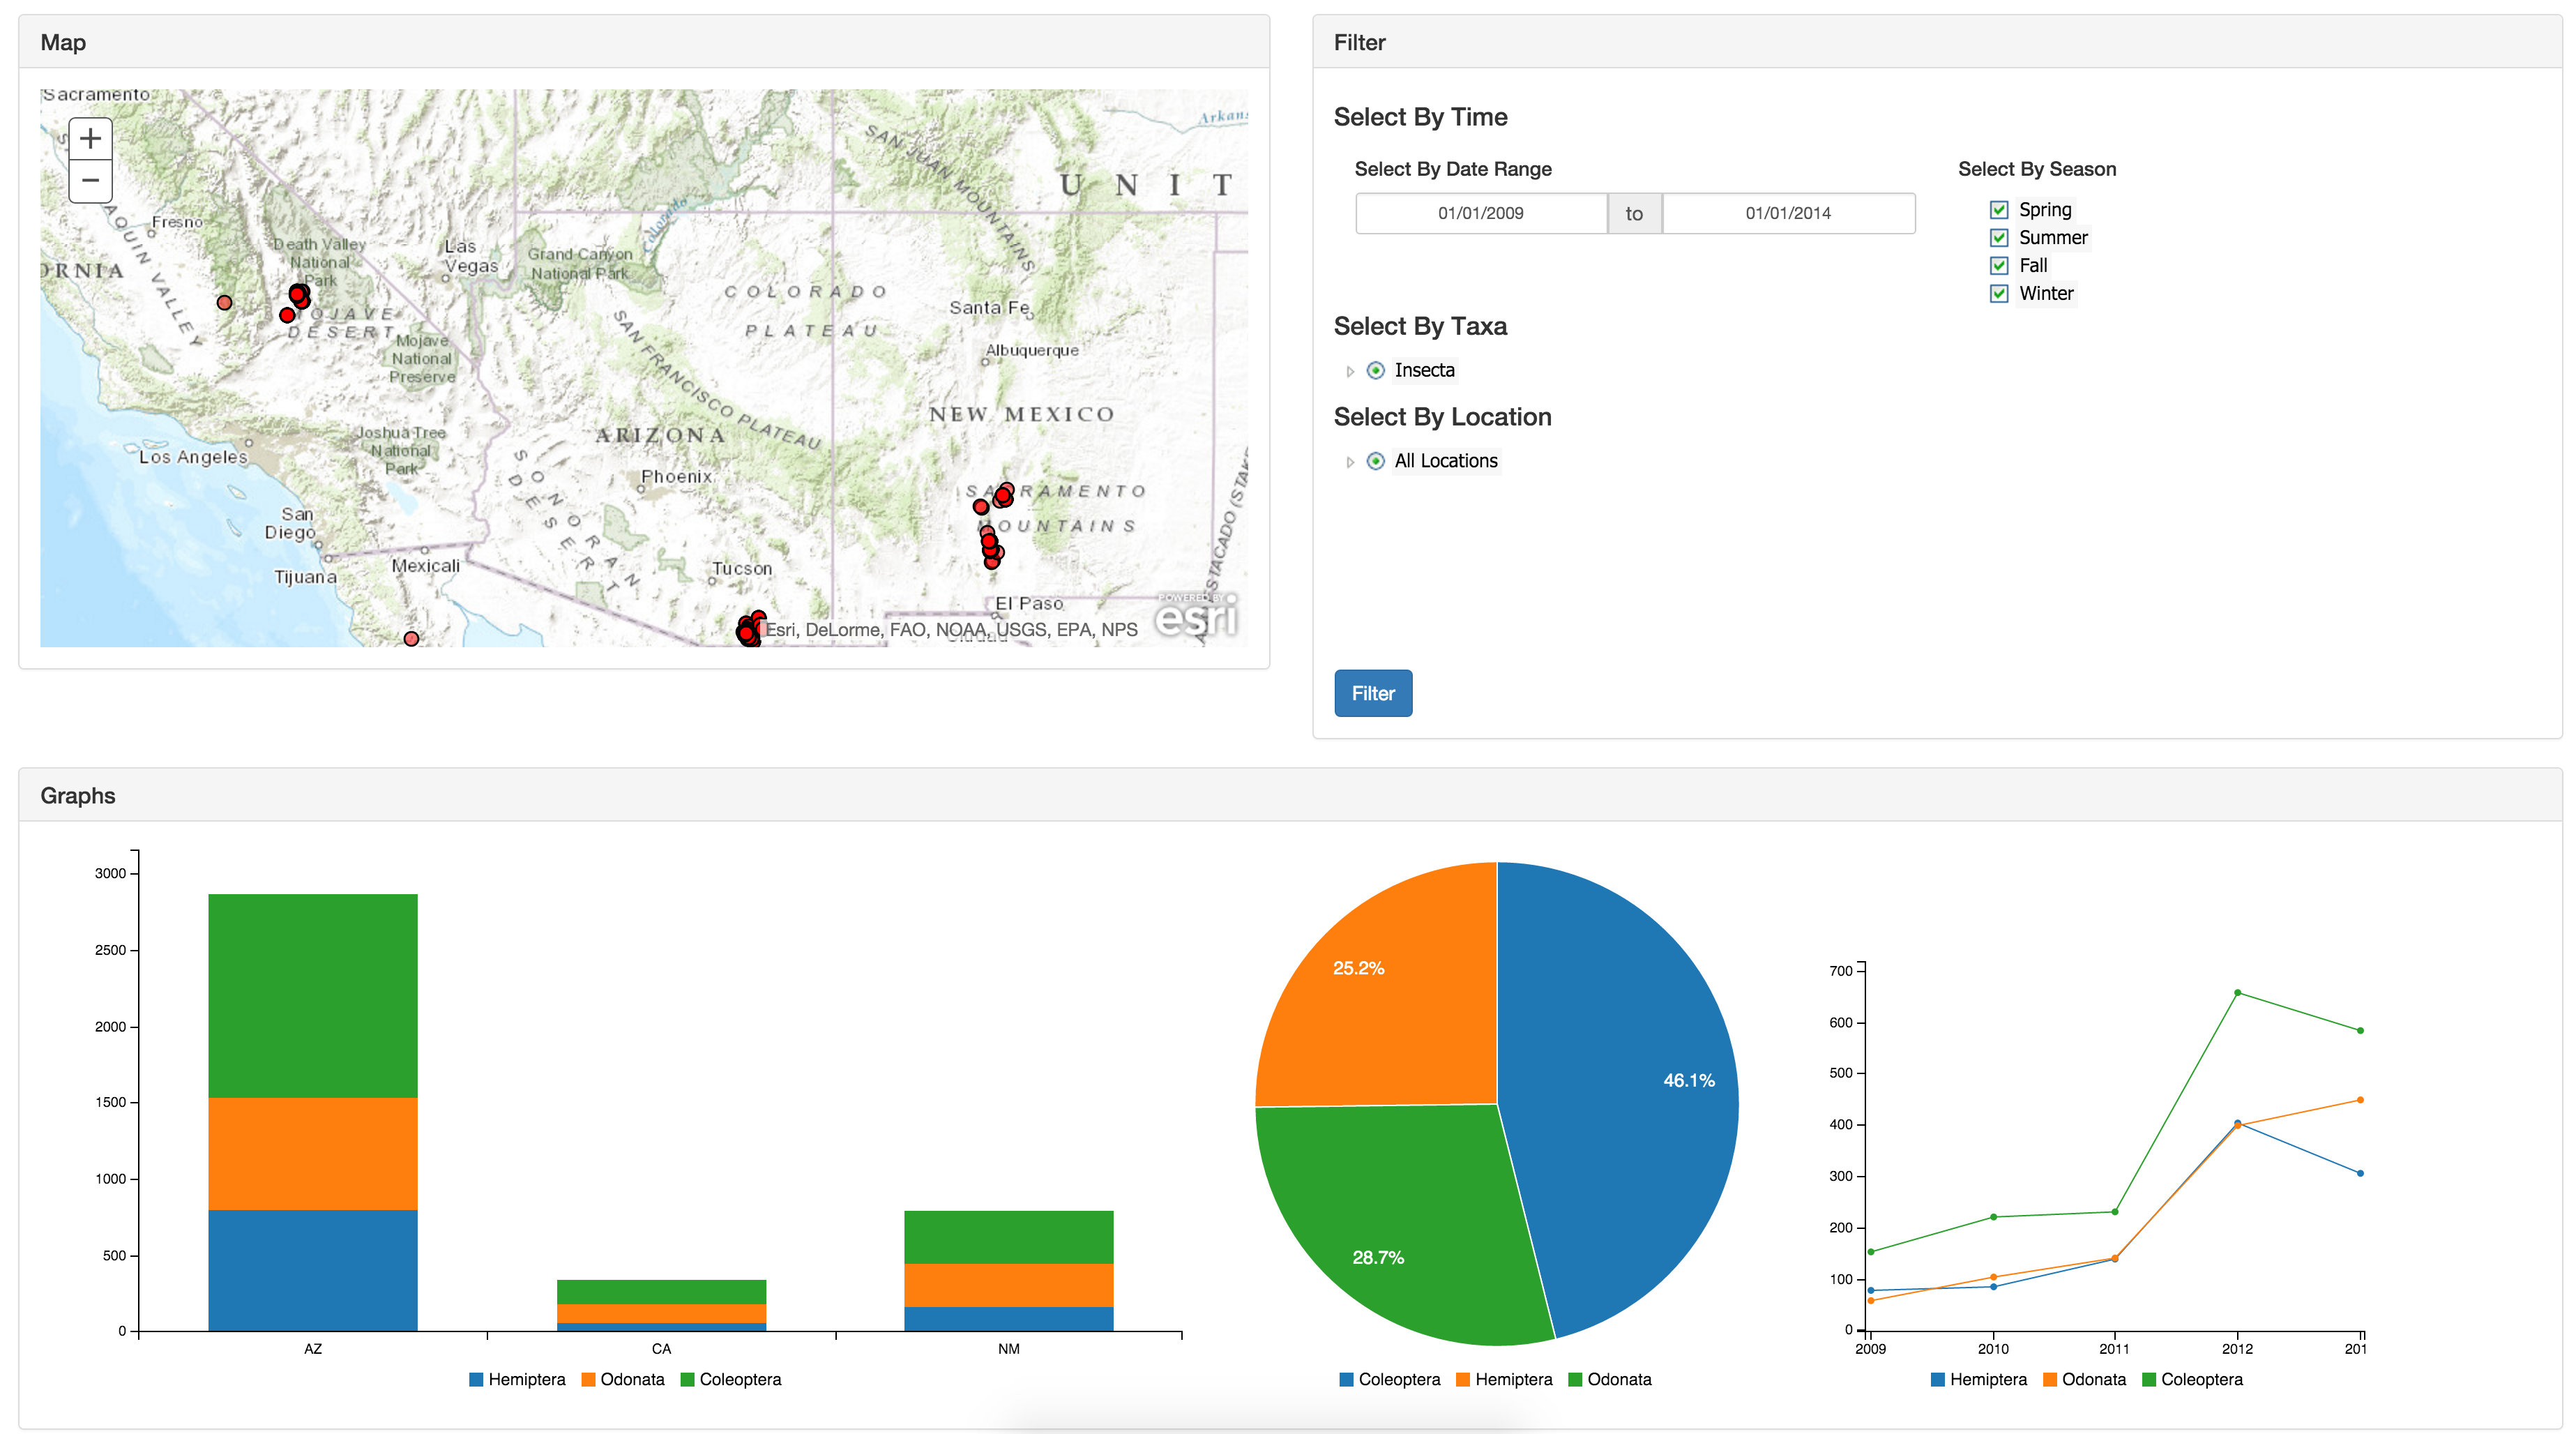
\includegraphics[width=0.45\textwidth]{images/figure_1.jpg}
\end{figure}

The main challenge with developing our single page web-app was providing data to the various tools we’re making use of in our different containers.
We have written models that map objects to database entries and allow us to provide serialized data to our templates.

\subsection{Filter View}
% @TODO: JASPER

\subsection{Map View}
% @TODO: ALEC

\subsection{Graph View} % @TODO: TY
The graph view portion of our web tool is alpha-level ready.
We have interactable example charts already deployed that render  static data.
A couple of them even have data being dynamically loaded into them from the database, but that wasn’t an alpha-level goal for us, so we are focusing on that for the beta release.
The particular statistics of interest haven’t been nailed-down yet, so our sponsor wanted us to have a proof-of-concept with just displaying how example graphs would look.
We are able to customize every aspect of them in regards to color, spacing, font, layout, etc.
An example of what the graph-portion looks like is shown above.
When the page is resized to be smaller, the graph window view will display a horizontal scroll bar so that the user can still see the metrics they’re interested in without having to scrunch them up.

\begin{figure}[h]
\caption{Graph View}
\centering
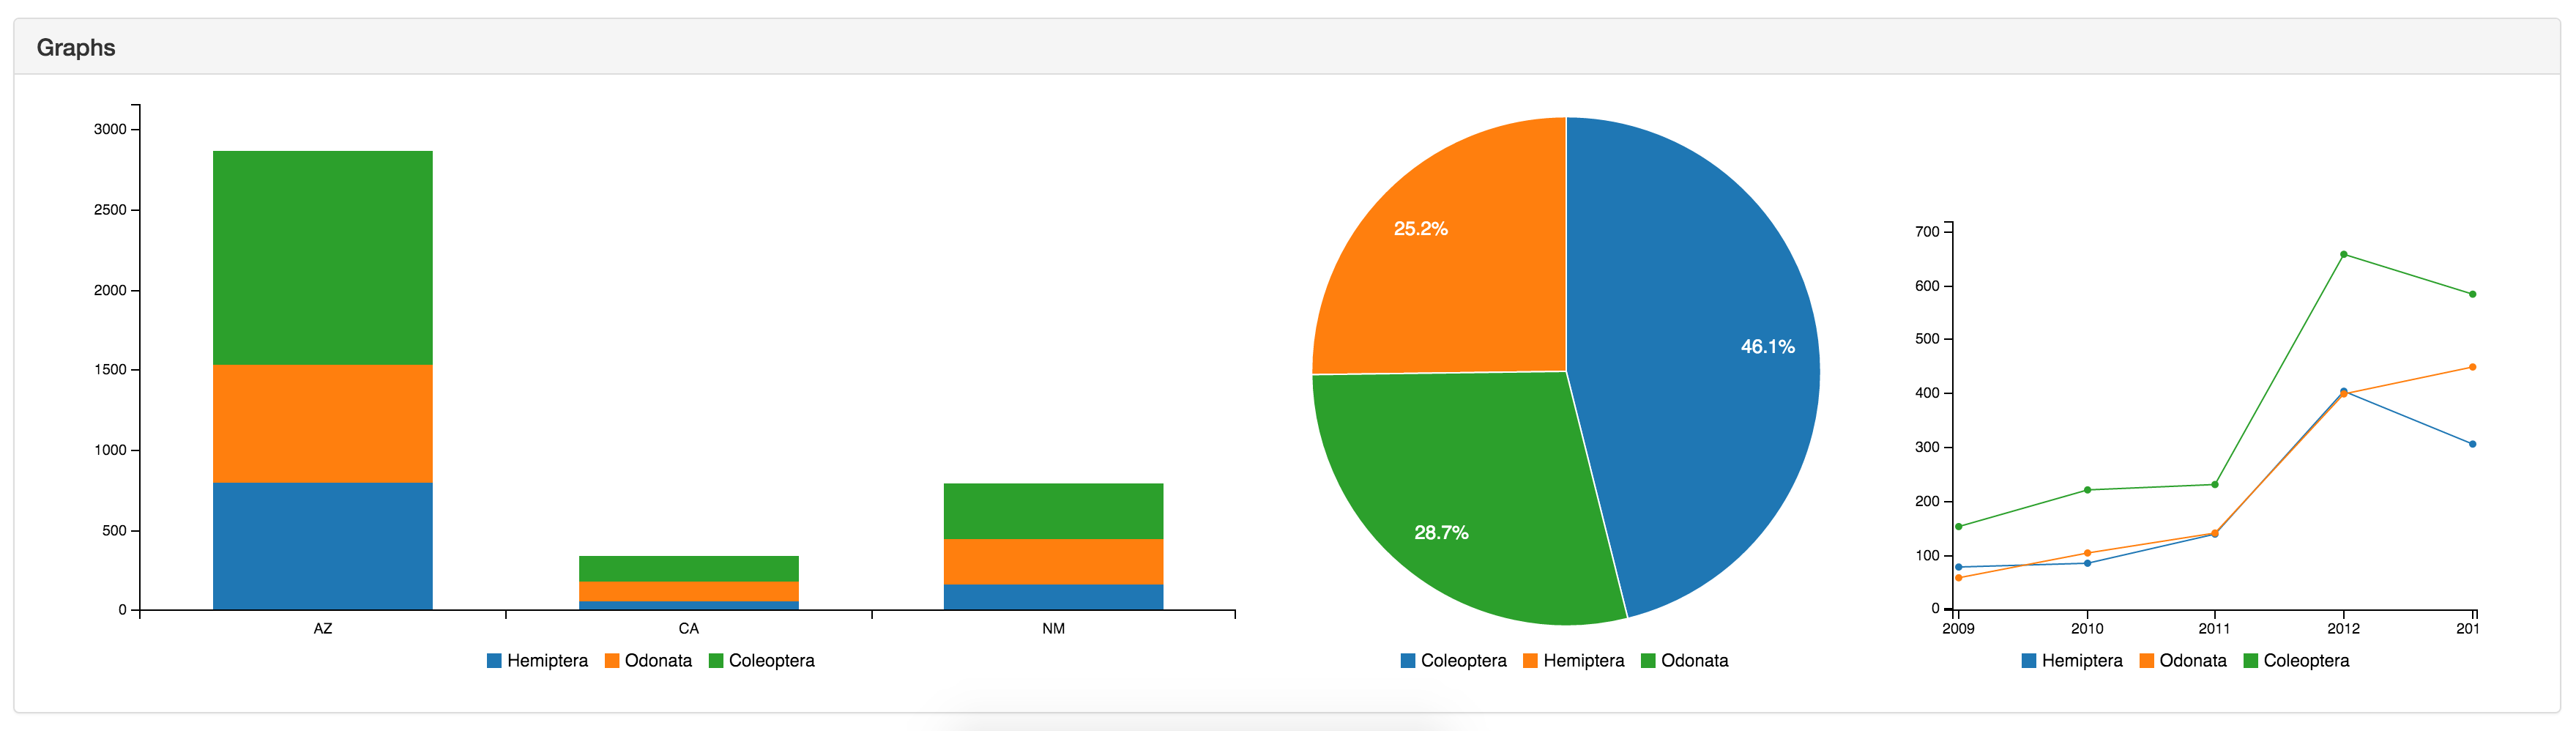
\includegraphics[width=0.45\textwidth]{images/figure_6.jpg}
\end{figure}

One of the graphs that we were successful in dynamically rendering data into was the pie-chart that displayed the number of biodiversity readings within a specific order.
Since this was just an attempt to render data from the database on-load, it’s not actually a graph that we will show when in production, because it could be specified for genus or species.
We just wanted to have the biodiversity distribution pie chart available for alpha along with some way to prove we could get data dynamically from the database.

\begin{figure}[h]
\caption{Pie chart showing order distribution}
\centering
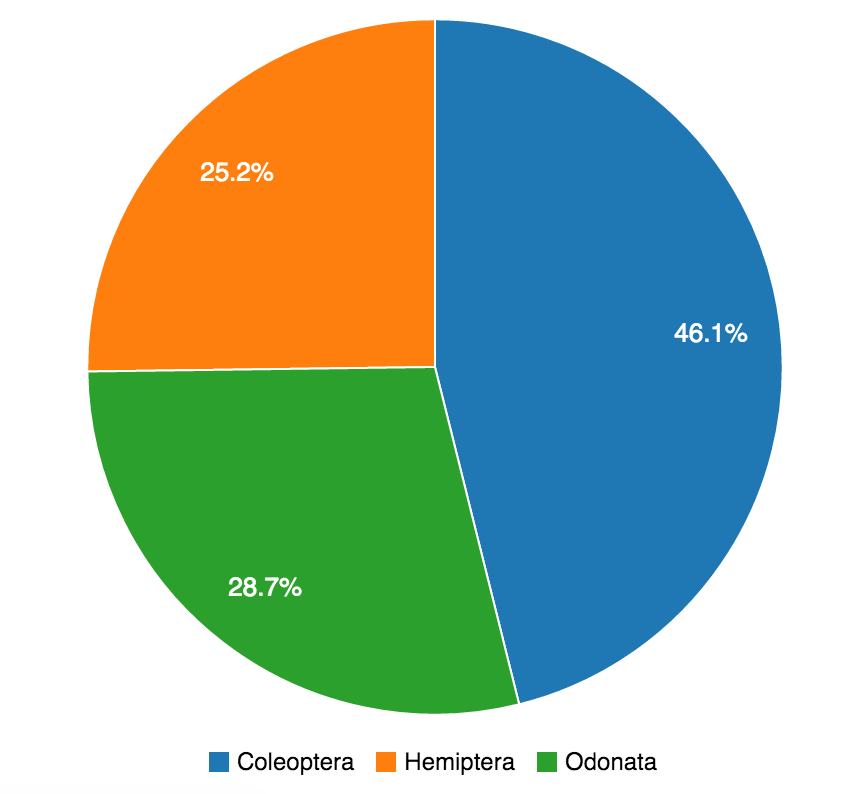
\includegraphics[width=0.25\textwidth]{images/figure_7.jpg}
\end{figure}

The graph below displays a functionality in c3 that is really useful and is one of the primary reasons that we chose c3 as our graphing library for development.
If the user is to click (or touch on a touchpad) the label for a particular dataset within a graph, then the graph will hide that dataset and focus on only the remaining.
This is a very important functionality, because when taking biodiversity readings there could be an under-represented species or genus that only shares a small percentage of the dataset.
There could even be multiple that are dominated by one large collection.
If the user wants to ‘zoom in’ on those particular small readings, they could just hide the dominating dataset by clicking its label.

\begin{figure}[h]
\caption{Showing the interactive pie chart}
\centering
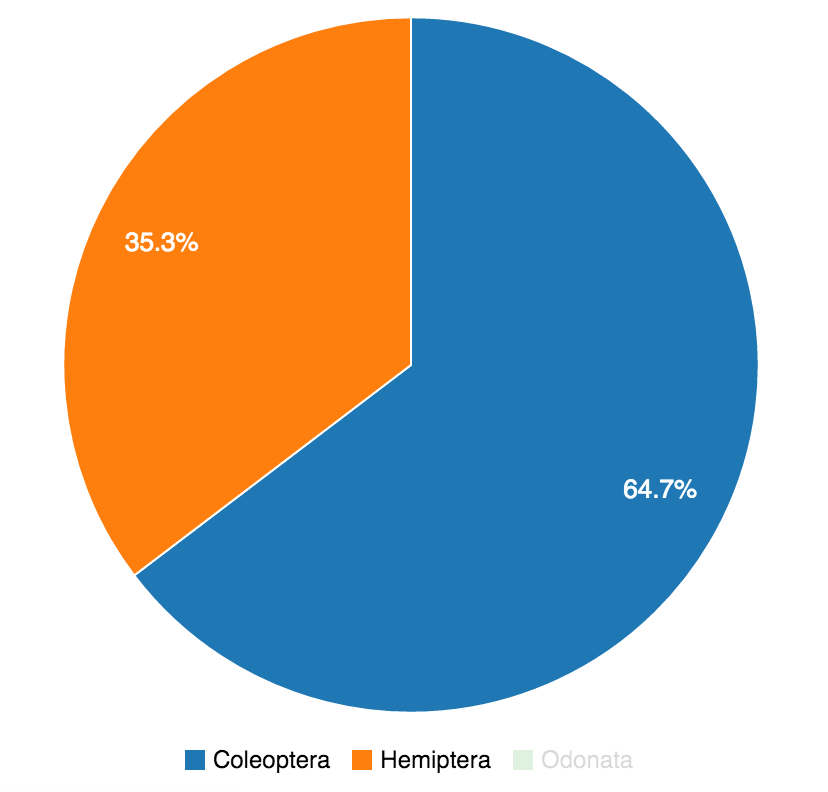
\includegraphics[width=0.25\textwidth]{images/figure_8.jpg}
\end{figure}

During development we encountered some varyingly-sized problems that slowed us down, but we were able to overcome them before alpha release.
Even though providing data to the graph view dynamically from the database was not a primary goal for the alpha, it was a very challenging process.
None of us have used Django in the past and its ORM (object relational mapping) model structure, for constructing and querying objects from the database, was completely foreign to us.
Once we were able to learn how Django does it’ s aggregate queries to the database it became a little bit more clear how to perform our queries, but it still proves to be challenging.
We were able to get the correct data to render in one or two graphs, but the process of getting exactly the data we need along with massaging it into the format required by c3 (and arcGIS, filter, etc.) is a challenge in itself as well.
Come beta release, we will be providing dynamic data to each template and hopefully filtering/interacting between them.

\subsection{Database and Preparing Data}
% @TODO: ALEC

\section{Remaining Work}

\subsection{Requests Between Views}
% @TODO: TY

\subsection{Filter to Graph}
% @TODO: TY

\subsection{Filter to Map}
% @TODO: ALEC

\subsection{What the Graph View Displays}
% @TODO: JASPER


\end{document}
